
\begin{frame}
    \frametitle{Locomoción}
    \small
    El humano copia a la naturaleza para construir tipos de locomoción.
    \TODO{Mostrar ejemplos del libro Figura 2.1. animales y robots reales.}

    \begin{center}
        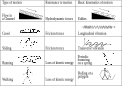
\includegraphics[width=0.7\columnwidth]{images/biological_locomotion_systems.pdf}
    \end{center}

    La naturaleza tuvo que adaptar a los animales para terrenos irregulares!

    \note{Los insectos por ejemplo tienen que sortear cambios de altura que superan en ordenes de magnitud su tamaño.}

    Utilizamos ruedas por que son muy eficientes en terrenos planos y firmes.
\end{frame}


\begin{frame}
    \frametitle{Locomoción}

    Manipulación: un brazo robótica está fijo y mueve objetos en su espacio de trabajo aplicando fuerza sobre ellos.

    Locomoción: el entorno está fijo y el robot se mueve impartiendo fuerza sobre el entorno.
    \begin{itemize}
        \item Estabilidad
        \begin{itemize}
            \item Geometría y Número de puntos de contacto
            \item Centro de gravedad
            \item Estabilidad estática y dinámica
            \item Inclinación del terreno
        \end{itemize}
        \item Característica de contacto
        \begin{itemize}
            \item Punto de contacto/ distancia y forma de camino
            \item Ángulo de contacto
            \item Fricción
        \end{itemize}
        \item Tipo de entorno
        \begin{itemize}
            \item Estructura
            \item Medio (agua, aire, terreno suave o firme)
        \end{itemize}
    \end{itemize}
\end{frame}

\begin{frame}
    \frametitle{Locomoción}
    Ventajas y desventajas de robots con patas:

    Ventajas: permite ir por terrenos irregulares, reducen el impacto ambiental dado que tienen menos puntos de contacto.
    Desventaja: complegidad mecánica, mayor consumo (una pata con muchos joints puede tener que bancar todo el paso del robot), para que tenga mucha maniobrabilidad cada las patas deben tener muchas juntas.

\end{frame}


\begin{frame}
    \frametitle{Gaits}

\end{frame}


\begin{frame}
    \frametitle{Tipos de Ruedas}

\end{frame}

\begin{frame}
    \frametitle{Drones?}

\end{frame}